%%%% CAPÍTULO 4 - RESULTADOS E DISCUSSÃO

\chapter{Resultados}\label{cap:resultados}

TODO

% Este capítulo apresenta o que foi obtido como resultado do trabalho, que, em princípio, é o sistema desenvolvido. Se não for um sistema, como, por exemplo, uma solução na área de redes, neste capítulo é reportada a solução proposta. Neste caso, a divisão do capítulo em seções é realizada, se necessária, de acordo com o trabalho.

% O capítulo pode conter seções de acordo com o tipo de sistema e a necessidade de documentação mais extensa de determinados aspectos. Caso o trabalho se refira à comparação entre tecnologias ou dados obtidos como resultados do uso do sistema, além da descrição do sistema, há os dados obtidos com os testes e a discussão desses dados. Nesse caso haverá uma seção para os dados obtidos desses testes e as discussões.

\section{Escopo do sistema}\label{sec:escopoSistema}

TODO

% Apresenta o escopo do sistema (contendo entre dois ou cinco parágrafos) de forma bastante sucinta, considerando aspectos técnicos e conceituais. O escopo define o que é o sistema, consistindo das funcionalidades e características que o sistema deve conter. É importante apresentar também o escopo negativo, ou seja, as funcionalidades e características que o sistema não irá conter. 
% Exemplo:

% O sistema XYZ deve gerenciar todos os processos de uma livraria virtual, desde a aquisição até a venda dos livros para o consumidor final. O acesso dos compradores e gerentes deve ser feito por meio de um site WEB, incluindo a possibilidade de acesso por outras tecnologias (ex. celular, tablet). Os clientes poderão fazem as compras pagando com cartão de crédito ou depósito bancário. Existem promoções eventuais pelas quais os livros podem ser comprados com desconto.

% De início, a livraria vai trabalhar apenas com livros novos a serem adquiridos de editoras que tenham sistema automatizado de aquisição. Desta forma, o sistema a ser desenvolvido deve conectar-se aos sistemas das editoras para efetuar as compras.

% O sistema deve calcular o custo de entrega baseado no peso dos livros e na distância do ponto de entrega. Eventualmente podem haver promoções do tipo “entrega gratuita” para determinadas localidades.

% O sistema deve permitir a um gerente emitir relatórios de livros mais vendidos, e compradores mais assíduos, bem como sugerir compras para compradores baseadas em seus interesses anteriores.

\section{Modelagem do sistema}\label{sec:modelagemSistema}

TODO

% A modelagem do sistema inclui os diagramas e as descrições textuais para representar o problema e a solução.

% Sendo assim, primeiramente esse item deve apresentar diagramas utilizados para a modelagem de negócios (ex. diagramas de atividade e estado), se esses tenham sido necessários.
% Em seguida esse item deve conter a descrição dos requisitos obtidos do usuário, contendo sua respectiva classificação (funcionais e não funcionais). Sugere-se o uso de um modelo formal sugerido por autores (ex. Wazlawick, Bezerra) para a apresentação dessa classificação.

% Se utilizada orientação a objetos e a UML, nesta seção ainda são apresentados, por exemplo, os diagramas de casos de uso, com suas descrições suplementares, os diagramas de classe de análise (ou modelo conceitual), de sequência e/ou comunicação, diagrama de classes de projeto.

% Nesta seção também estão os diagramas da modelagem de banco de dados, como entidade-relacionamento. Nesse item pode ser apresentada a descrição de cada uma das classes do modelo de classes apresentado acima, assim como a descrição das tabelas do banco de dados. Também podem estar documentados modelos e padronizações utilizados para a interface, diagramas de navegação, a representação da arquitetura do sistema e dos padrões de projeto utilizados.

\section{Apresentação do sistema}\label{sec:apresentacaoSistema}

TODO

% Apresenta as funcionalidades e o uso de recursos tecnológicos do sistema por meio de suas telas, enfatizando a interação com o sistema. A apresentação do sistema é feita sob a forma de texto, com telas e definição de padrões que forem relevantes ao contexto do trabalho. As telas são tratadas como figuras, cópias (print screen) de relatórios ou consultas também são figuras.

% A \autoref{fig:cadastroPaciente} exibe a tela de acesso ao Cadastro de Pacientes.

% \begin{figure}[htpb]%% Ambiente figure
% \captionsetup{width=0.43\textwidth}
% \caption{Tela de acesso ao Cadastro de Pacientes.}%% Legenda
% \label{fig:cadastroPaciente}%% Rótulo
% 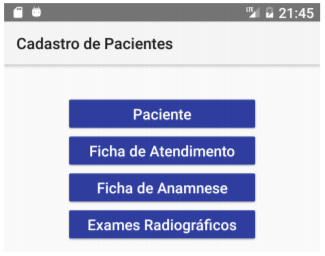
\includegraphics[scale=0.8]{cadastro-paciente}%% Dimensões e localização
% \fonte{}%% Fonte
% \end{figure}

\section{Implementação do sistema}\label{sec:implementacaoSistema}

TODO

% Nesta seção é documentada a implementação do sistema com partes relevantes ou exemplos de código, rotinas, funções. Inclui, ainda, a descrição técnica do uso de recursos (componentes, bibliotecas, etc.) da linguagem. Ressalta-se que cada orientador avaliará juntamente com seu orientado o que poderá ser descrito nesta seção. Isso sem que sejam revelados detalhes do sistema que possam comprometer seu uso comercial ou científico ou que a descrição fique muito sucinta ou superficial.

% Em materiais e método estão quais os recursos utilizados, neste capítulo é reportado como esses recursos foram utilizados para resolver o problema.

% Sugere-se colocar listagens curtas de código, enfatizando aspectos específicos das tecnologias utilizadas ou da implementação. Sugere-se, ainda, que o código não seja apresentado sob a forma de print screen, e sim copiado e colado no texto, mantendo, se possível, a formatação. Todas as listagens de código devem ser devidamente explicadas. A explicação deve ser técnica, fundamentada em aspectos conceituais e boas práticas de programação.

% Enfatizar os diferenciais do sistema: procedimentos armazenados, consultas SQL, uso de componentes, uso de padrões de projeto, a forma de uso dos recursos da linguagem. Esses diferenciais são no sentido de explicitar as vantagens, desvantagens, dificuldades e facilidades que esses recursos impetraram no desenvolvimento do sistema em termos técnicos. Esses diferenciais servirão para avaliar pela utilização ou não desses recursos, pelo menos para sistemas iguais ou semelhantes ao reportado no trabalho.

% Reportar a forma como o sistema foi verificado e validado. No sentido de verificar se os requisitos definidos para o mesmo foram atendidos. Os testes podem ser realizados pelo professor orientador, pelos professores que compõem a banca, por pessoas que serviram de base para as informações para o sistema e etc. Os testes podem ser realizados com base em um plano de testes elaborado juntamente com a análise e projeto do sistema. Para validar a implementação podem ser desenvolvidas rotinas de teste unitário.

% Se houver implantação do sistema, mesmo que seja para teste, reportar a forma como isso foi feito, a geração de instaladores, os problemas com ambiente e sistema operacional, incluindo banco de dados e outros. Deixar explícito o procedimento para instalar e usar o sistema.

% Quando for necessário, citar no texto do trabalho nomes de campos, tabelas ou rotinas específicas utilizadas na implementação de um software, utilizar a fonte courier new para destacar esses nomes.

% Um exemplo de listagem de código fonte pode ser observado na \autoref{codigo:classeFoo}, que representa a classe Aluno.

% \begin{sourcecode}[htb]
% \caption{\label{codigo:classeFoo}Classe Aluno}
% \begin{lstlisting}[frame=single, language=Java]
% @Entity
% public class Foo {
 
%     @Id
%     @GeneratedValue(strategy = GenerationType.IDENTITY)
%     private Long id;
 
%     private String nome;
    
%     private Integer ra;
     
%     // constructor, getters and setters
% }
% \end{lstlisting}
% \fonte{}
% \end{sourcecode}

\section{Implantação do sistema}\label{sec:implantacaoSistema}

TODO

\section{Discussões}\label{sec:discussoes} 

TODO

% O trabalho contém esta seção quando considerado que há resultados (em termos de dados) e discussões relevantes ou suficientes para justificar uma seção. Se existentes e não justificarem uma seção, eles podem estar na seção que relata a implementação do sistema.

% Nesta seção estão os resultados obtidos da realização de testes quantitativos e qualitativos, independentemente da quantidade, tipo e volume de testes realizados. Os resultados dos testes são discutidos tendo como base o referencial teórico e os objetivos pretendidos com o trabalho. Esses testes podem resultar de implantação e testes de uso do sistema. 

\section{Trabalhos Relacionados}\label{sec:trabalhosRelacionados} 

O trabalho desenvolvido por \citet{qoselearning} realiza uma análise quantitativa do impacto de parâmetros de conexão de rede em ambientes de ensino remoto sustentados por uma estrutura de \textit{VDI}. A análise é feita a partir de um experimento com o objetivo de clarificar a relação entre a qualidade de conexão com a internet e a usabilidade de sistemas de ensino remoto.

O resultado do experimento mostrou que é possível realizar atividades como escrita, desenhos e consumo de mídias, sem grandes prejuízos para a usabilidade, mas é necessário que a conexão com a internet tenha qualidade. Outro ponto importante é que fora atividades de visualização de vídeos, a largura de banda não é um fator de grande consumo nesses tipos de ambientes.

Outro trabalho de grande relevância para essa produção, desenvolvido por \citet{edufirestick}, apresenta um sistema de \textit{VDI} para educação remota utilizando as mesmas tecnologias propostas no presente trabalho. 

A proposta da produção é de criar uma \textit{VDI} de baixo custo com Instâncias EC2 Spot\footnote{Instâncias EC2 Spot são máquinas virtuais oferecidas pela AWS em um modelo de precificação mais barato que o modelo comum, utilizando o excedente de capacidade computacional} da \textit{AWS} e com o Apache Guacamole para gerenciamento das conexões, e permitindo o acesso de qualquer dispositivo com um navegador de internet, até mesmo televisões smart, como apresentado no trabalho.

A solução proposta por \citet{edufirestick} aborda um cenário de aula de laboratório, onde um professor pode agendar um evento de criação das máquinas virtuais para os alunos e no horário da aula, todos poderiam acessar o recurso reservado para a aula.

Em termos de custos operacionais, o trabalho apresenta uma estimativa de custo por usuário de USD\$ 0.87 mensais com a utilização dos seguintes parâmetros:

\begin{itemize}
    \item Tempo de conexão diária: 18 horas
    \item Categoria da instância: t3.micro
    \item Sistema operacional: \textit{Microsoft Windows Server 2019}
    \item Memória: 4 GB de RAM
    \item Espaço em disco: 90 GB
    \item Região: São Paulo
\end{itemize}

Em termos de preço pela transferência de dados, o trabalho relata um custo de USD\$ 0.06 por hora em picos onde o uso de banda chaga a 2 MB/s. O custo dos outros serviços que suportam a infraestrutura, foi estimado em USD\$ 200.00 mensais.

O trabalho feito por \citet{edufirestick} apresenta um panorama muito promissor e consoante aos objetivos do presente trabalho, demostrando que é possível executar a solução em um cenário de laboratório. Mas ainda não apresenta resultados referentes ao gerenciamento de \textit{desktops} que tenham os dados persistidos, para outros cenários de uso, como o de pesquisa por exemplo.